\documentclass[11pt, a4paper]{article}
\usepackage{graphicx}
\usepackage{amsmath}
\usepackage{listings}
\usepackage{minted}
\usepackage{physics}

\title{EE2703 Applied Programming Lab - Assignment No 6}
\author{
  \textbf{Name}: Atishay Ganesh\\
  \textbf{Roll Number}: EE17B155
}\date{\today}
\begin{document}
		
\maketitle 
\section{Abstract}
The goal of this assignment is the following.
\begin{itemize}
\item To analyze LTI Systems using Laplace Transform.
\item To see how RLC systems can be used as a low pass filter .
\item To understand how to use the scipy signals toolkit.
\item To plot graphs to understand the Laplace Transform.
\end{itemize}
\usemintedstyle{manni}

\section{Assignment}
\subsection{Setting up the variables}
Importing the standard libraries
\begin{minted}[mathescape,escapeinside = ||]{python3}
import numpy as np
import matplotlib.pyplot as plt
import scipy.signal as sp
import matplotlib
\end{minted}
We define a plotting function to help simplify the code.
\begin{minted}{python3}
def plotter(fig_no,arg1,arg2,
    label_x,label_y,type=plt.plot,
    arg3='b-',title="",cmap = matplotlib.cm.jet):
    '''plotter function to help with standard plots'''
    plt.figure(fig_no)
    plt.grid()
    if type==plt.contourf:
        type(arg1,arg2,arg3,cmap=cmap)
        '''mostly only contour graphs use a colormap'''
        plt.colorbar()
    else:
        type(arg1,arg2,arg3)
    plt.xlabel(label_x,size =19)
    plt.ylabel(label_y,size =19)
    plt.title(title)
\end{minted}
We also define a function to make bode plots.
\begin{minted}{python3}
def bodeplot(w,s,phi):
    '''Makes Bode Plots'''
    plt.subplot(2,1,1)
    plt.semilogx(w,s)
    plt.xlabel(r'$\omega$',size=17)
    plt.ylabel(r'$|H(j\omega)|$',size =17)
    plt.subplot(2,1,2)
    plt.semilogx(w,phi)
    plt.xlabel(r'$\omega$',size=17)
    plt.ylabel(r'$\angle(H(j\omega))$',size =17)
\end{minted}
\subsection{Single Spring System}
\subsubsection{Varying the Decay of the Input}
{
We use the Laplace transform to solve a simple spring system.
The system is characterized by the given differential equation.
\[\dv[2]{x}{t} + 2.25x = f(t) \]
(Initial Conditions all zero)
whose Laplace transform is of the form
\[H(s) =  \frac{1}{s^2+2.25}\]
The input signal is of the form 
\(f(t) = \cos{(\omega t)}\exp(-at)u(t)\),
where a is the decay factor and $\omega$ is the frequency of the cosine.\\
The Laplace Transform of the input signal is
\[ F(s) = \frac{s+a}{(s+a)^2+\omega^2 }\]
First we define these function these using numpy polynomials and multiply to get the output laplace transform.
Finally we take the ILT of the function using sp.impulse to get the time domain sequences and we plot these.
We do this for $\omega$=1.5 (natural frequency of the system), and decay of 0.5 and 0.05.
}
\begin{minted}{python3}
def input_fn(decay=0.5,cos_term=1.5):
    '''input function to the single spring system'''
    return (np.poly1d([1,decay]),
    np.poly1d([1,2*decay,cos_term**2+decay**2]))

def transfer_fn():
    '''transfer function of the single spring system'''
    return (np.poly1d([1]), np.poly1d([1,0,2.25]))

def input_td(t,freq,decay):
    '''time domain expression of a generalised
     input to the spring system'''
    return(np.cos(freq*t)*np.exp(-1*decay*t))

def solve(decay):
    '''using the convolution property of the laplace 
    transform to solve for the output of the LTI system'''
    Hn, Hd = transfer_fn()
    Fn, Fd = input_fn(decay)
    np.polymul(Fn,Hn)
    t = np.linspace(0,50,200)
    Y = sp.lti(np.polymul(Fn,Hn),np.polymul(Fd,Hd))
    t, y = sp.impulse(Y,None,t)
    plotter(1,t,y,"t","x(t)",
        title="System response with decay {}".format(decay))
    plt.show()

#High decay rate
solve(0.5)
#Low decay rate
solve(0.05)

\end{minted}
\begin{figure}[!tbh]
   	\centering
   	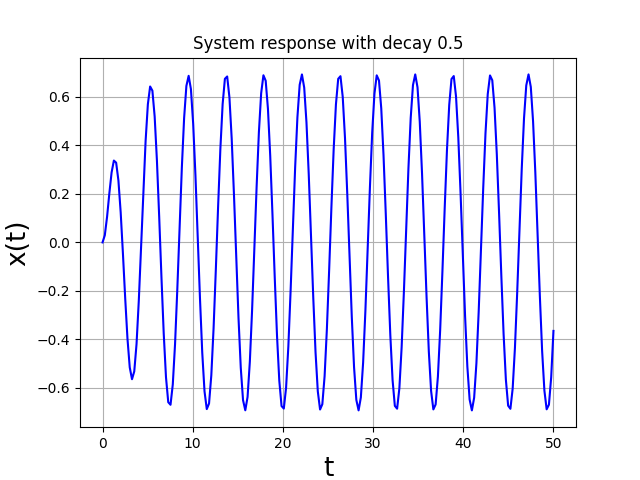
\includegraphics[scale=0.5]{img1.png}
   	\label{fig:32}
   \end{figure}
\begin{figure}[!tbh]
   	\centering
   	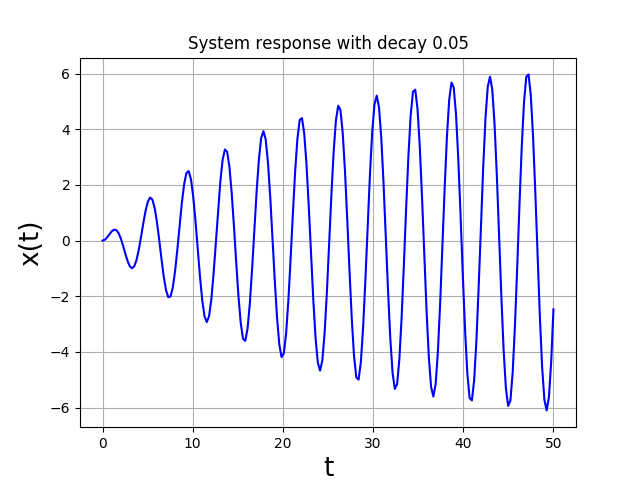
\includegraphics[scale=0.5]{img2.png}
   	\label{fig:32}
   \end{figure}
{
We observe that the osciallation amplitude settles to  a fixed value in both the cases.
We observe it takes longer to settle with decay being less.
We also observe that the amplitude increases to a much larger amount in the case with lower decay.
At zero (or negative) decay the amplitude increases ad infinitum, and at high decay it reaches the max amplitude almost instantaneously.
}
\subsubsection{Varying the frequency of the input}
{
We vary the frequency of the cosine  and see what affect it has on the output.
We also construct the bode plot of the transfer function to better understand the results. 
}
\begin{minted}{python3}
def loop_freq(decay = 0.05):
    '''This function shows the plot  at various frequencies
    and also calculates the bode plot parameters'''
    t = np.linspace(0,100,300)
    Hn,Hd = transfer_fn()
    H = sp.lti(Hn,Hd)
    color_list=['k','g','r','c','m']
    # Short forms for colors
    # Black Green Red Cyan and Magenta
    fl = np.arange(1.4,1.6,0.05)
    
    for i in range(5):
        u = input_td(t,fl[i],decay)
        t,y,svec = sp.lsim(H,u,t)
        plotter(1,t,y,"t","x(t)",
                title="System response with decay 0.05 and various frequencies",
                arg3=color_list[i]+'-')
    plt.legend(["freq {}".format(i) for i in fl])
    plt.show()
    return(H.bode())


w,s,phi = loop_freq()
#Making a bode plot to better understand 
#the variation of the response with the input frequency.
bodeplot(w,s,phi)
plt.title('Bode plot of Transfer function of spring system')
plt.show()

\end{minted}
\begin{figure}[!tbh]
   	\centering
   	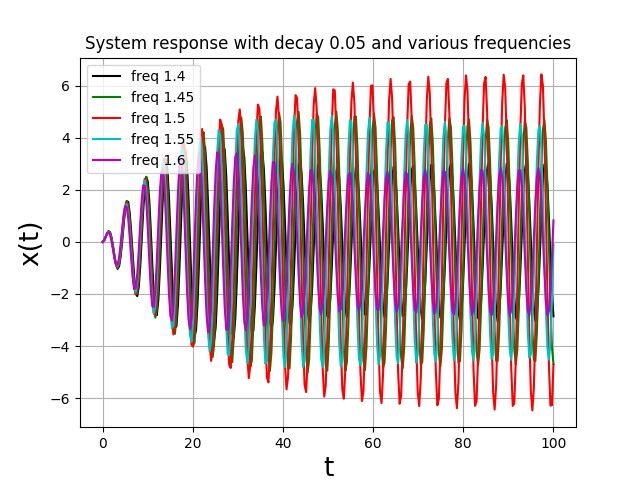
\includegraphics[scale=0.5]{img3.png}
   	\label{fig:32}
   \end{figure}
\begin{figure}[!tbh]
   	\centering
   	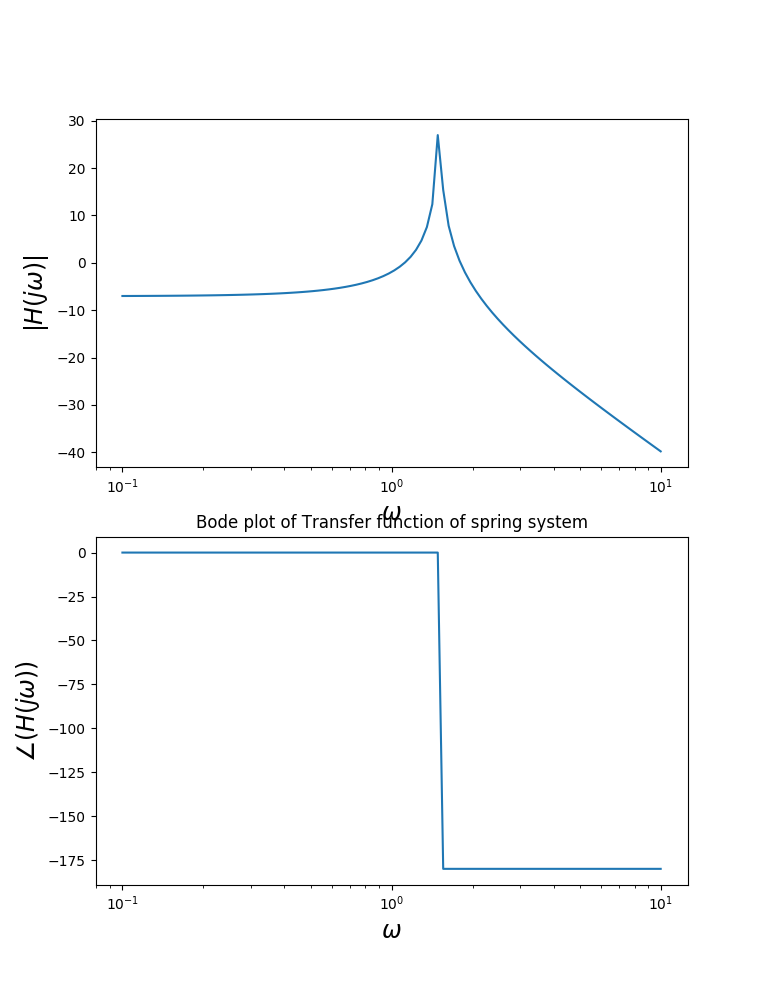
\includegraphics[scale=0.5]{img4.png}
   	\label{fig:32}
   \end{figure}
{
When the input frequency is at the natural frequency the output amplitude is maximum.
In the other cases the output amplitude decreases.
This phenomenon is known as resonance.
We can see clear from the bode plot that there is a maximum at the natural frequency, as there is a second order pole there.
The phase shift is -180$\deg$, which agrees with the fact that the pole is in the left half plane.
}
\subsection{Coupled Spring Problem}
{
In this problem we have two differential equations and two variables to solve for.
The equations are
\[\dv[2]{x}{t} +(x-y) = 0 \]
\[\dv[2]{y}{t} +2(y-x) = 0 \]
With initial condition as x(0) = 1
We substitute for y in the second equation from the first, and we get a fourth order differential equation in terms of x.
Simplifying this and substituting to find the y equation, we get.
\[X(s) = \frac{s^2+2}{s^3+3s} \]
\[Y(s) =  \frac{2}{s^3+3s} \]
We can take the ILT of these two expressions to find the time domain expressions for x(t) and y(t).
We plot these in 1 graph.
}
\begin{minted}{python3}
def coupled():
    '''solving the coupled springs problem'''
    t = np.linspace(0,20,200)
    #Transfer function for X
    X = sp.lti([1,0,2],[1,0,3,0])
    #Transfer function for Y
    Y = sp.lti([2],[1,0,3,0])
    t,x = sp.impulse(X, None, t)
    t,y = sp.impulse(Y, None, t)
    plotter(1,t,x,"t","f(t)",title="Coupled Spring system, plot of x")
    plotter(1,t,y,"t","f(t)",title="Coupled Spring system, plot of y",arg3 ="g-")
    plt.legend(["f(t) = x(t)","f(t) = y(t)"])
coupled()
plt.show()

\end{minted}
\begin{figure}[!tbh]
   	\centering
   	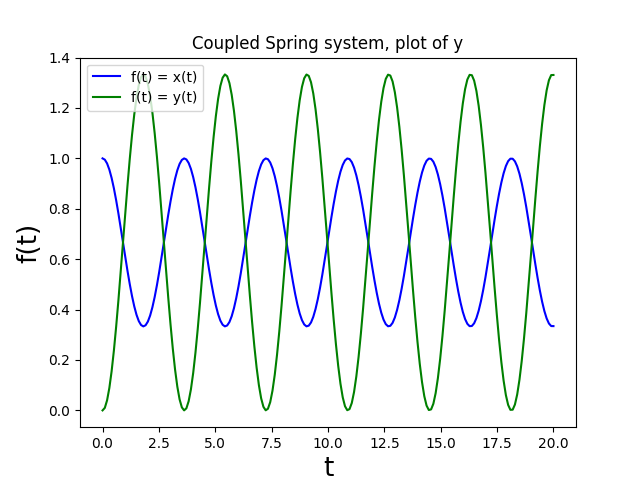
\includegraphics[scale=0.5]{img5.png}
   	\label{fig:32}
   \end{figure}
{ 
We observe that the amplitude of y is greater than x. 
The phase of the two are opposite.
The offsets are the same for both the expressions.
This models two masses attached to the ends of an ideal spring.
}
\subsection{RLC Filter}
{
We now consider the case of an RLC Filter with the transfer function as shown.
\[ H(s) = \frac{1}{10^{-12}s^2 + 10^{-4}s + 1}\]
(Initial Conditions all zero)
The input is of the form
\[x(t) = \cos{(10^3t)}+\cos{(10^6t)} \]

which is basically the superposition of two sinusoids with low and high frequencies.
First we plot the bode plot of the transfer function.
Then we use sp.lsim to find the output of the filter to the input system.
We plot the output from 0 to 30$\mu$s as well as from 0 to 10ms.
}
\begin{minted}{python3}
def rlc_tf():
    '''Transfer function for the RLC Circuit'''
    return(np.poly1d([1]),np.poly1d([1e-12,1e-4,1]))

def rlc_input(t):
    '''Input to the RLC Circuit'''
    return(np.cos(1e3*t)-np.cos(1e6*t))

def solve_rlc():
    '''RLC Solver'''
    t = np.arange(0,10e-3,1e-7)
    Hn,Hd = rlc_tf()
    H = sp.lti(Hn,Hd)
    #Plotting the Bode plot for the RLC Circuit
    w,s,phi = H.bode()
    bodeplot(w,s,phi)
    plt.title('Bode plot of Transfer function of RLC Filter')
    plt.show()
    #Solving the RLC Circuit
    u = rlc_input(t)
    t,x,svec = sp.lsim(H,u,t)
    
    plt.rcParams.update({'mathtext.default':  'regular' })
    plotter(1,t,x,"t","V(t)",
    title="RLC Circuit, plot of output Voltage, Slow Time")
    plotter(2,t[0:300],x[0:300],"t","V(t)",
    title="RLC Circuit, plot of output Voltage, Fast Time")

    plt.ylabel('$V_{o}(t)$')
    plt.show()
solve_rlc()

\end{minted}
\begin{figure}[!tbh]
   	\centering
   	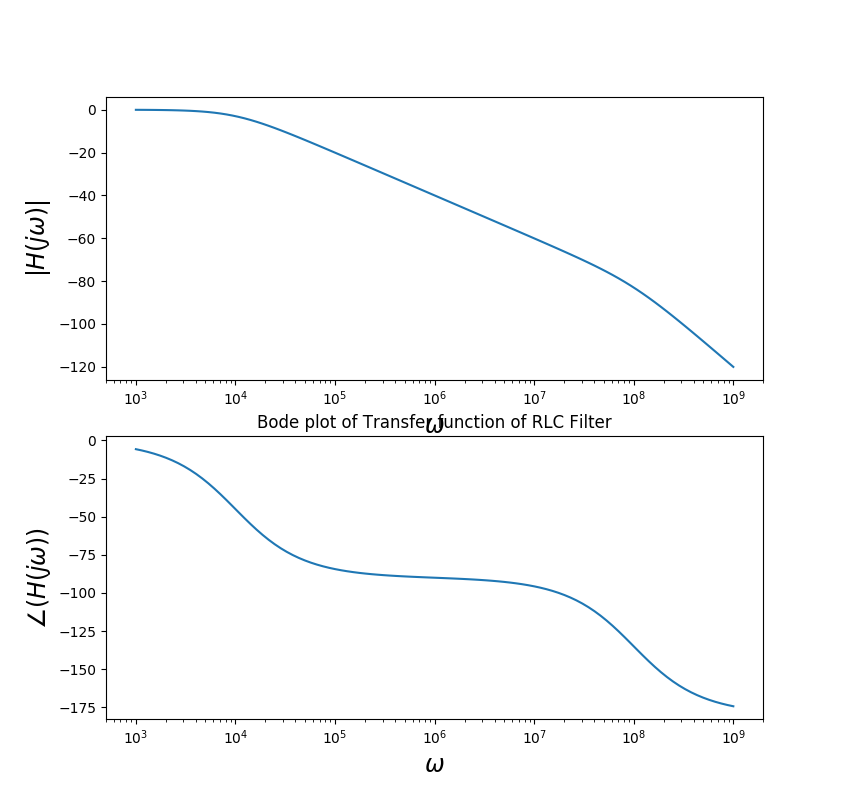
\includegraphics[scale=0.5]{img6.png}
   	\label{fig:32}
   \end{figure}
\begin{figure}[!tbh]
   	\centering
   	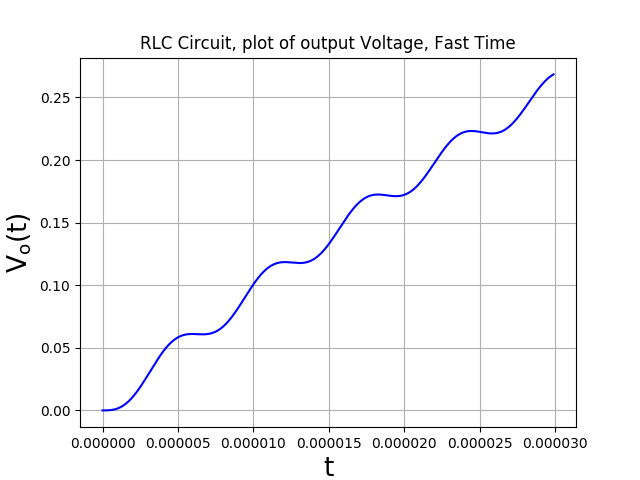
\includegraphics[scale=0.5]{img7.png}
   	\label{fig:32}
   \end{figure}
\begin{figure}[!tbh]
   	\centering
   	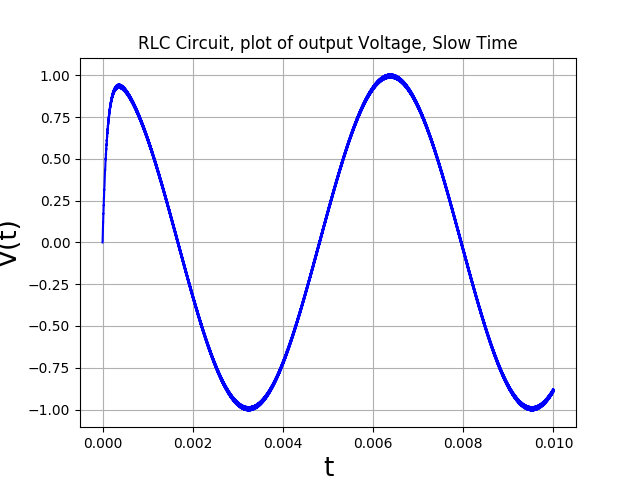
\includegraphics[scale=0.5]{img8.png}
   	\label{fig:32}
   \end{figure}
{
From the Bode plot, it is clear that the RLC System is a second order low pass filter, with the 3db bandwidth of 
The slow time plot shows that the capacitor is charging up to meet the input amplitude. The high frequency component can be seen as a ripple in the slow time plot.  This component is highly attenuated and hence not visible in the fast time plot.
In the fast time plot, we see that the low frequency component passes almost unchanged, the amplitude is almost 1.
The reason is that the $\omega = 10^3\frac{rad}{s}$ is well within the 3-dB bandwidth ($\omega_{3dB} = 10^4\frac{rad}{s}$) of the system.
Clearly this reiterates the fact that this is a low pass filter with bandwidth $\omega_{3dB} = 10^4\frac{rad}{s}$.

}

\section{Conclusions}
\begin{itemize}
\item We  analyzed LTI Systems using Laplace Transform.
\item We saw a low pass filter constructed from an RLC circuit.
\item We used the scipy signals toolkit to calculate the time domain response and the Bode Plot.
\item We plotted graphs to understand the above
\end{itemize}

\end{document}